%---------------------------------------------------------
% Plantilla para un seminario con Beamer
%---------------------------------------------------------

\documentclass[dvipsnames, pdflatex,slidecentered]{beamer}
\usepackage{xcolor,colortbl}
\usepackage{hyperref}
\hypersetup{colorlinks=true, urlcolor=brown}
%  options  [handout]


%Posibles alternativas:
%\usetheme{Boadilla}
%\usetheme{default}
\usetheme{CambridgeUS}
\usecolortheme{lily}
%-------------------------------------------------------------
% Colors
\definecolor{yellowgreen}{rgb}{0.6,0.8,0.2}
\definecolor{firebrick1}{rgb}{1,0.19,0.19}
\definecolor{lightgray}{rgb}{0.83,0.83,0.83}
\definecolor{gray51}{rgb}{0.51,0.51,0.51}
\definecolor{gray31}{rgb}{0.31,0.31,0.31}
%\mode<presentation>{
%\useinnertheme{rounded}
%\usefonttheme[onlymath]{serif}
%\useleftsidebartemplate{0.5cm}{}
%\userightsidebartemplate{0.5cm}{}
%}
\usepackage[utf8]{inputenc}
%----------------------------------------------------------------------
% Para que aparezcan varias transparencias en la misma p\'{a}gina
\usepackage{pgfpages}
%\pgfpagesuselayout{4 on 1}[a4paper,border shrink=5mm,landscape]
%----------------------------------------------------------------------
% Suprime los s\'{\i}mbolos de navegaci\'{o}n
\setbeamertemplate{navigation symbols}{}
%---------------------------------------------------------------------

%\usepackage{amsmath,amssymb}

%--------------------------------------------------------------------------------------
%----------------------------------------------------------------
\newcommand{\ep}{\epsilon}
\newcommand{\real}{{\rm I\kern-.17em R}}
\newcommand{\pro}{\mbox{P}}
%-----------------------------------------------------------------

\title[Estad\'{\i}stica: Tema 6]{Tema 6\\
Extensiones y aplicaciones\\
(Máquinas de vectores soporte, SVM)}
\author[Berrendero]
{Jos\'{e} R. Berrendero}
\date{}
\institute{Departamento de Matem\'{a}ticas\\
 Universidad Aut\'{o}noma de Madrid}

%-------------------------------------------------------------------------------------------
\begin{document}
\begin{frame}[plain]

\vspace{2cm}
\titlepage

%\begin{minipage}{5cm}
%\vspace{-15.8cm}
%\hspace{-2cm}
%\centerline{\scalebox{0.4}{\includegraphics{figures/def5bis}}}
%\end{minipage}

\end{frame}
%----------------------------------------------------------------------
\begin{frame}[plain]
\frametitle{Contenidos del tema 6}

\begin{itemize}
 

  \item El problema de clasificación supervisada: un ejemplo
  \item SVM para datos separables linealmente.
  \item SVM para datos no separables linealmente.
  \item Reglas de clasificación no lineales: el truco del núcleo.

  
 
\end{itemize}


\end{frame}
%---------------------------------------------------------------------
\begin{frame}[plain]
\frametitle{Diagnóstico por imagen del cáncer de mama}

\begin{minipage}{5cm}
\begin{itemize}
\item Punción con aguja fina.
\item La muestra se tiñe para resaltar los núcleos de las células.
\item Se determinan los límites exactos de los núcleos.
\item Las variables corresponden a distintos aspectos de su forma. 
\end{itemize}
\end{minipage}
\begin{minipage}{5cm}
\centerline{{\includegraphics[width=5cm]{imagen}}}
\end{minipage}

\end{frame}
%---------------------------------------------------------------------
\begin{frame}[plain]
\frametitle{Variables}

\begin{tabular}{|c|c|}
\hline
\textbf{nombre} & \textbf{descripción} \\ \hline
radius & radio del núcleo \\
texture & varianza de los niveles de gris en el interior del núcleo \\
perimeter & perímetro del núcleo\\
area & área del núcleo\\
smoothness & suavidad medida mediante la variación del radio\\
compactness & el perímetro al cuadrado dividido por el área\\
concavity & medida de la importancia de las concavidades \\
concavepoints & número de concavidades\\
symmetry & medida de la simetría del núcleo\\
fractal & dimensión fractal de la frontera \\ \hline
\end{tabular}

\

 \begin{center}
 \href{http://archive.ics.uci.edu/ml/}{Más información sobre estos datos}
 \end{center}

\end{frame}
%---------------------------------------------------------------------
%\begin{frame}[plain]
%\frametitle{Diagramas de dispersión}

%\begin{center}
%\includegraphics[scale=0.4]{wbc-pairs}
%\end{center}

%\end{frame}
%---------------------------------------------------------------------
\begin{frame}[plain]
\frametitle{Gráfico de estrellas}

\begin{center}
\includegraphics[scale=0.4]{wbc-stars}
\end{center}

\end{frame}
%---------------------------------------------------------------------
\begin{frame}[plain]
\frametitle{Variables \textit{smoothness} y \textit{concavepoints}}

\begin{center}
\includegraphics[scale=0.3]{wbc2-dispersion}
\end{center}

\end{frame}
%-----------------------------------------------
\begin{frame}[plain]
\frametitle{Clasificación supervisada}

Disponemos de una muestra de datos bien clasificados (\textit{training data}):

\[
(x_1,y_1),\ldots, (x_n,y_n)
\]
donde $x_i\in \mathbb{R}^d$ son las variables observadas e $y_i\in\{-1,1\}$ es la etiqueta que representa la clase a la que pertenecen las observaciones.

\

Se observa ahora un nuevo vector $x$ independiente de los anteriores.

El objetivo es determinar a qué clase pertenece la observación $x$.

\

La regla óptima (regla Bayes) consiste en asignar a $x$ el valor $y=1$ si y solo si
\[
\mathbb{P}(y=1| x) > \mathbb{P}(y=-1|x)
\]
No es aplicable en la práctica.

\end{frame}
%---------------------------------------------------------------------
\begin{frame}[plain]
\frametitle{SVM para datos separables linealmente}

\begin{itemize}
\item Suponemos que las muestras de ambos grupos son separables mediante un hiperplano.

\begin{center}
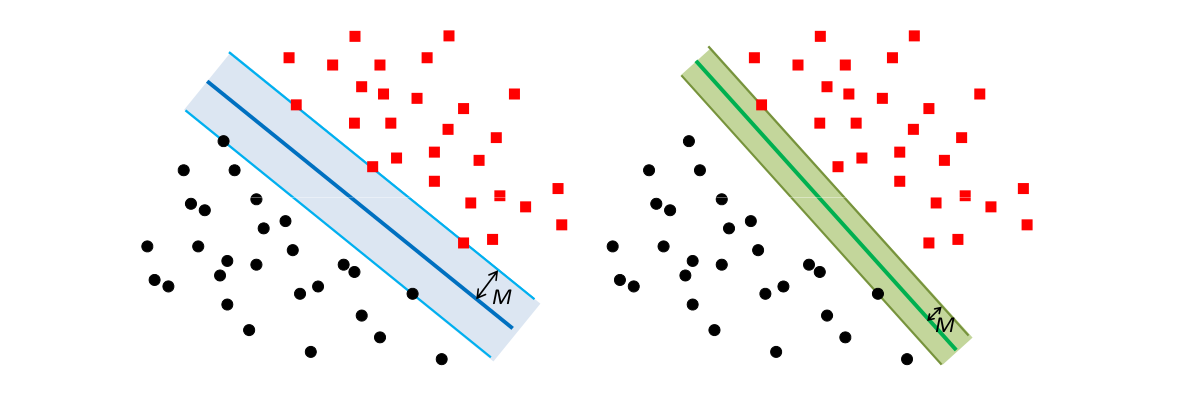
\includegraphics[scale=0.7]{margen}
\end{center}

\item El \textbf{margen} de un hiperplano separador viene dado por la menor distancia de los puntos al hiperplano. 

 \item El \textbf{hiperplano óptimo} es aquel que maximiza el margen.

\end{itemize}

\end{frame}
%---------------------------------------------------------------------
\begin{frame}[plain]
\frametitle{Distancia de un punto a un hiperplano}

\begin{itemize}



\item Distancia de un punto $x$ al hiperplano $w' x + w_0=0$.

\

Sea $\hat x$ el punto del hiperplano más cercano a $x$. Entonces,
\[
x = \hat x + r \frac{w}{\|w\|} \Rightarrow w' x + w_0 = (w' \hat x + w_0) + r \|w\| = r \|w\|.
\]

\

\item La distancia de un punto $x$ al hiperplano es:
\[
d = |r| = \frac{|w' \hat x + w_0|}{\|w\|}.
\]

\end{itemize}



\end{frame}
%---------------------------------------------------------------------
\begin{frame}[plain]
\frametitle{Margen}

\begin{itemize}


\item Disponemos de una muestra de datos clasificados $(x_i,y_i)$, $i=1,\ldots, n$.

\item La clase es $y_i\in\{-1,1\}$.

\

\item Un hiperplano separador verifica $y_i(w'x_i+w_0)>0$, para todo $i=1,\ldots,n$.

\item Siempre podemos definir $w$ y $w_0$ de manera que 
\[
\min_i \{y_i(w' x_i + w_0)\}=1.
\]

\

\item El margen es
\[
\mbox{Margen} = \min_i  \frac{y_i(w' x + w_0)}{\|w\|} = \frac{1}{\|w\|}.
\]

\end{itemize}

\end{frame}

%---------------------------------------------------------------------
\begin{frame}[plain]
\frametitle{Hiperplano separador óptimo}

\begin{itemize}

\item Buscamos el hiperplano separador que maximiza el margen.



\

\item Tenemos que resolver el problema convexo

\begin{center}
\begin{tabular}{lll}
minimizar & $\|w\|^2 / 2$ \\
s.a. & $y_i(w' x_i + w_0)\geq 1$,  &  $i=1,\ldots,n$
\end{tabular}
\end{center}

\

\item La función lagrangiana de este problema es
\[
L(w,w_0) = \frac{\|w\|^2}{2} - \sum_{i=1}^n u_i[y_i(w'x_i+w_0)-1] 
\]

\end{itemize}

\end{frame}
%---------------------------------------------------------------------
\begin{frame}[plain]
\frametitle{Condiciones KKT}

Las condiciones de Karush-Kuhn-Tucker que debe satisfacer la solución de este problema son:

\



\begin{itemize}
\item El gradiente de la función lagrangiana se anula



\item Se cumplen las restricciones del problema



\item Los multiplicadores no son negativos.



\item Se cumplen las condiciones de holgura complementaria.

\end{itemize}

\

Estas condiciones permiten deducir algunas propiedades importantes de la solución.

\end{frame}
%---------------------------------------------------------------------
\begin{frame}[plain]
\frametitle{Condiciones KKT}

\[
\nabla L(\hat w,\hat w_0) = 0 \Rightarrow \hat w = \sum_{i=1}^n \hat u_i y_i x_i\ \ \ \mbox{y}\ \  \  \sum_{i=1}^n \hat u_i y_i = 0.
\]


Para $i=1,\ldots, n$,
\[
y_i(\hat w' x_i + \hat w_0)\geq 1, \ \ \hat u_i\geq 0
\]


\[
\hat u_i\big( y_i(\hat w' x_i + \hat w_0) - 1\big) = 0
\]

\

El hiperplano óptimo solo depende de aquellos puntos de los que está más cerca ($ y_i(\hat w' x_i + \hat w_0) > 1\Rightarrow \hat u_i=0$). 

\


Típicamente son pocos. Se llaman \textbf{vectores soporte}.

\end{frame}
%--------------------------------------------------------------------
\begin{frame}[plain]

\begin{center}
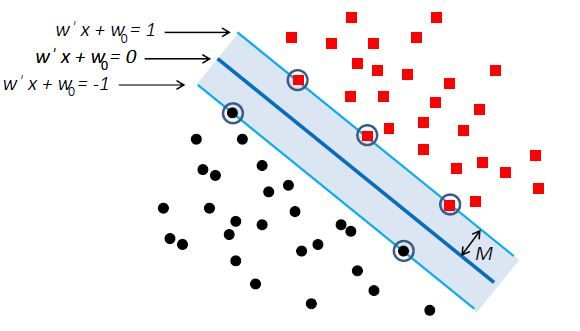
\includegraphics[scale=0.7]{soporte.jpg}
\end{center}

\end{frame}
%---------------------------------------------------------------------
\begin{frame}[plain]
\frametitle{Problema dual}

\begin{itemize}

\item \textbf{Función dual} (se obtiene minimizando la función lagrangiana en $w$ y $w_0$):
\[
g(u) =  \sum_{i=1}^n u_i - \frac{1}{2} \sum_{i=1}^n \sum_{j=1}^n 
u_i u_j y_i y_j x'_i x_j 
\]
si $\sum_{i=1}^n  u_i y_i = 0$, y $g(u)=-\infty$ en caso contrario.

\

\item \textbf{Problema dual}:

\

\begin{center}
\begin{tabular}{lll}
maximizar & $g(u)$ \\
s.a. & $\sum_{i=1}^n  u_i y_i = 0$.  & \\
& $u_i\geq 0,\ \ i=1,\ldots,n$.
\end{tabular}
\end{center}



\end{itemize}

\end{frame}
%---------------------------------------------------------------------
\begin{frame}[plain]
\frametitle{Problema dual}

En forma matricial, si  $\mathbf{1}_n=(1,\ldots,1)'\in\mathbb{R}^n$, $y=(y_1,\ldots,y_n)'$ y $H$ es la matriz cuyas entradas son $h_{ij}=y_iy_jx_i'x_j$, 


\begin{center}
\begin{tabular}{ll}
maximizar & $u'\mathbf{1}_n - \frac{1}{2}u'Hu$ \\
s.a.     &  $u'y=0$ \\
     & $u\geq 0$.    
\end{tabular}
\end{center}


\begin{itemize}

\item Es un problema de optimización convexo (la matriz $H$ es definida positiva).

\item La solución depende de $x_1,\ldots,x_n$ únicamente a  través de los productos escalares $x'_ix_j$.

\end{itemize}


\end{frame}
%-----------------------------------------------
\begin{frame}[plain]
\frametitle{Cálculo del hiperplano óptimo}

\begin{itemize}
\item Resolvemos el problema dual mediante algún método de programación convexa estándar.

\

\item A partir de la solución del dual, $\hat u$, aplicamos $\hat w = \sum_{i=1}^n \hat u_i y_i x_i$ para obtener $\hat w$.

\

\item Sean $S=\{i:\, \hat u_i>0\}$ los índices de los vectores soporte.
Por las condiciones de holgura complementaria,  para cada $i\in S$,
\[
\hat w_0 = \frac{1-y_i\hat w'x_i}{y_i} = y_i-\hat w'x_i.
\] 

\

\item En la práctica, es numéricamente más estable usar el promedio de estos valores. Si $\# S=n_s$.
\[
\hat w_0 = \frac{1}{n_s} \sum_{i\in S} (y_i-\hat w'x_i).
\]
\end{itemize}


\end{frame}
%-----------------------------------------------
\begin{frame}[plain]
\frametitle{Regla de clasificación}

Resulta una regla de clasificación lineal: asignamos a $x$ el valor $y=1$ si y solo si $\hat{w}'x+\hat w_0>0$.

\

\[
\hat w_0 + \hat{w}'x>0 \Leftrightarrow \hat w_0 + \left[\sum_{i\in S} y_i \hat u_i x_i\right]' x > 0 
\]

\

Si $\alpha_i=y_i\hat u_i$, también podemos escribir la regla de clasificación como:
\[
y = 1 \Leftrightarrow  \hat w_0 + \sum_{i\in S} \alpha_i (x'_ix)>0
\]

¿Cómo afecta a la clasificación una rotación de los datos?

\end{frame}
%-----------------------------------------------
\begin{frame}[plain]
\frametitle{SVM para datos no separables linealmente}

En la práctica, la mayoría de los datos no son separables linealmente.

\

Se introducen unas variables de holgura $\xi_1,\ldots,\xi_n$ de manera que:

\begin{itemize}
\item se relajan las restricciones con el fin de permitir errores de clasificación,
\item se cambia el objetivo para penalizar estos errores.
\end{itemize}

\

\begin{center}
\begin{tabular}{lll}
minimizar & $\|w\|^2 / 2 + C\sum_{i=1}^n \xi_i$ \\
s.a. & $y_i(w' x_i + w_0) + \xi_i\geq 1$,  &  $i=1,\ldots,n$\\
& $\xi_i\geq 0$,  &  $i=1,\ldots,n$
\end{tabular}
\end{center}

\

La constante $C>0$ es seleccionada por el usuario y determina si los errores se penalizan más o menos.

\end{frame}
%-----------------------------------------------
\begin{frame}[plain]
\frametitle{SVM para datos no separables linealmente}

\begin{center}
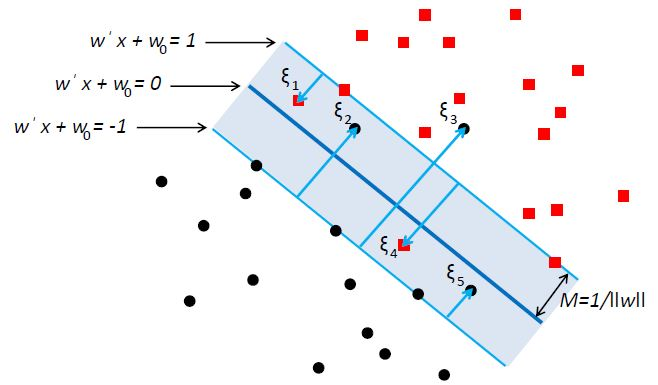
\includegraphics[scale=0.7]{holgura.jpg}
\end{center}


\end{frame}
%-----------------------------------------------
\begin{frame}[plain]
\frametitle{Condiciones KKT}



\[
L(w,w_0,u,v) = \frac{\|w\|^2}{2} +C\sum_{i=1}^n \xi_i - \sum_{i=1}^n u_i[y_i(w'x_i+w_0)+\xi_i-1] - \sum_{i=1}^n v_i\xi_i
\]

\

\begin{itemize}
\item Gradiente de $L$ igual a cero:
\[
 w = \sum_{i=1}^n  u_i y_i x_i;\ \  \sum_{i=1}^n u_i y_i=0.
\]

\item Factibilidad primal y dual:
\[
y_i(w' x_i + w_0) + \xi_i\geq 1;\ \ \xi_i\geq 0;\ \ 0\leq u_i\leq C.
\]

\item Holgura complementaria: 
\[
u_i[y_i(w' x_i + w_0) + \xi_i - 1]=0;\  \ (C-u_i)\xi_i =0.
\]
\end{itemize}




\end{frame}
%-----------------------------------------------
\begin{frame}[plain]
\frametitle{Cuestiones}

\begin{itemize}
\item Escribe la función y el problema dual. ¿Qué diferencias se observan respecto al caso en que los datos son separables linealmente?

\

\item ¿Qué condición deben verificar en este caso los vectores soporte?

\

\item Si $\hat u_i$, $i=1,\ldots, n$ es la solución del problema dual, ¿cómo se calculan $\hat w$ y $\hat w_0$

\

\item Escribe la regla de clasificación.

\end{itemize}

\end{frame}
%-----------------------------------------------
\begin{frame}[plain]
\frametitle{Ejemplo. SVM para datos no separables linealmente}

\begin{center}
\includegraphics[height=7cm,width=11cm]{svm-lineal}
\end{center}


\end{frame}
%-----------------------------------------------
\begin{frame}[plain]
\frametitle{Extensión a reglas no lineales}

\begin{center}
\includegraphics[scale=0.5]{nolineal.jpg}
\end{center}

\end{frame}
%-----------------------------------------------
\begin{frame}[plain]
\frametitle{Extensión a reglas no lineales}

\begin{itemize}
\item Es posible que una regla de clasificación lineal no sea apropiada para los datos originales $x_1,\ldots,x_n$ pero sí para los datos transformados $\phi(x_1),\ldots,\phi(x_n)$, donde $\phi:\mathbb{R}^d\to \mathcal{H}$ para un espacio de Hilbert $\mathcal{H}$.

\

\item Basta sustituir $x'_ix_j$ por $\langle \phi(x_i),\phi(x_j)\rangle_{\mathcal{H}}$ en el problema dual.

\

\item Típicamente $\mathcal{H}=\mathbb{R}^N$ con $N>>d$ o $\mathcal{H}$ es un espacio de funciones (dimensión infinita).

\

\item En la práctica, puede ser  difícil  calcular los productos escalares  $\langle \phi(x_i),\phi(x_j)\rangle_{\mathcal{H}}$.
\end{itemize}

\end{frame}
%-----------------------------------------------
\begin{frame}[plain]
\frametitle{El truco del núcleo (\textit{the kernel trick})}

\textbf{Teorema:} Una función $k:\mathbb{R}^d\times \mathbb{R}^d\to\mathbb{R}$ es simétrica y semidefinida positiva (SDP) si y solo si existe un espacio de Hilbert $\mathcal{H}$ y una transformación $\phi:\mathbb{R}^d\to \mathcal{H}$ tal que $k(x,y)=\langle \phi(x),\phi(y)\rangle_{\mathcal{H}}$.

\

\begin{itemize}
\item Estas funciones simétricas y SDP se llaman núcleos.

\

\item En la práctica, en lugar de elegir $\mathcal{H}$ y $\phi$, se elige un núcleo y se sustituye $x'_ix_j$ por $k(x_i,x_j)$.

\

\item Así se obtienen reglas de clasificación de la forma:
\[
y = 1 \Leftrightarrow  \hat w_0 + \sum_{i\in S} \alpha_i k(x_i,x) > 0.
\]
\end{itemize}

\end{frame}
%-----------------------------------------------
\begin{frame}[plain]
\frametitle{Algunos núcleos muy utilizados}

\begin{itemize}
\item Polinomios de grado $m$:
\[
k(x,y) = (x'y + c)^m.
\]

\item Gaussiano:
\[
k(x,y) = \exp\left(-\frac{\|x-y\|^2}{2\sigma^2} \right)
\]


\item Laplaciano:
\[
k(x,y) = \exp\left(-\frac{\|x-y\|}{\sigma}\right)
\]
\end{itemize}

Para cada problema concreto hay que usar un núcleo apropiado.

 Un polinomio de grado pequeño o el núcleo gaussiano suelen ser buenas primeras opciones.

\end{frame}
%-----------------------------------------------
\begin{frame}[plain]
\frametitle{Regla de clasificación con núcleo cuadrático}



\begin{center}
\includegraphics[height=7.5cm]{svm-cuadratico-sim}
\end{center}



\end{frame}
%-----------------------------------------------
\begin{frame}[plain]
\frametitle{Regla de clasificación con núcleo cuadrático}



\begin{center}
\includegraphics[height=7.5cm]{svm-cuadratico-sim-b}
\end{center}


Resultado para un núcleo cuadrático con $C=100$, $m=2$ y $c=1$
\end{frame}
%-----------------------------------------------

\begin{frame}[plain]
\frametitle{Regla de clasificación con núcleo cuadrático}



\begin{center}
\includegraphics[height=7.5cm]{svm-cuadratico}
\end{center}


Resultado para un núcleo cuadrático con $C=100000$, $m=2$ y $c=1$
\end{frame}
%----------------------------------------------------------------------
\end{document}
%----------------------------------------------------------------------

%-----------------------------------------------
\begin{frame}[plain]
\frametitle{}

\end{frame}
%----------------------------------------------

